\documentclass[report,gutter=10mm,fore-edge=10mm,uplatex,dvipdfmx]{jlreq}

\usepackage{lmodern}
\usepackage{amssymb,amsmath}
\usepackage{ifxetex,ifluatex}
\usepackage{actuarialsymbol}
\usepackage[]{natbib}
\RequirePackage{plautopatch}

% maru suji ① etc.
\usepackage{tikz}
\newcommand{\cir}[1]{\tikz[baseline]{%
\node[anchor=base, draw, circle, inner sep=0, minimum width=1.2em]{#1};}}

\usepackage{comment}

\begin{comment}

\ifnum0\ifxetex1\fi\ifluatex1\fi=0 % if pdftex
  \usepackage[T1]{fontenc}
  \usepackage[utf8]{inputenc}
  \usepackage{textcomp} % provide euro and other symbols
\else % if luatex or xetex
  \usepackage{unicode-math}
  \defaultfontfeatures{Scale=MatchLowercase}
  \defaultfontfeatures[\rmfamily]{Ligatures=TeX,Scale=1}
\fi
% Use upquote if available, for straight quotes in verbatim environments
\IfFileExists{upquote.sty}{\usepackage{upquote}}{}
\IfFileExists{microtype.sty}{% use microtype if available
  \usepackage[]{microtype}
  \UseMicrotypeSet[protrusion]{basicmath} % disable protrusion for tt fonts
}{}
\makeatletter
\@ifundefined{KOMAClassName}{% if non-KOMA class
  \IfFileExists{parskip.sty}{%
    \usepackage{parskip}
  }{% else
    \setlength{\parindent}{0pt}
    \setlength{\parskip}{6pt plus 2pt minus 1pt}}
}{% if KOMA class
  \KOMAoptions{parskip=half}}
\makeatother
\usepackage{xcolor}
\IfFileExists{xurl.sty}{\usepackage{xurl}}{} % add URL line breaks if available
\IfFileExists{bookmark.sty}{\usepackage{bookmark}}{\usepackage{hyperref}}
\hypersetup{
  hidelinks,
  pdfcreator={LaTeX via pandoc}}
\urlstyle{same} % disable monospaced font for URLs
\usepackage{longtable,booktabs}
% Correct order of tables after \paragraph or \subparagraph
\usepackage{etoolbox}
\makeatletter
\patchcmd\longtable{\par}{\if@noskipsec\mbox{}\fi\par}{}{}
\makeatother
% Allow footnotes in longtable head/foot
\IfFileExists{footnotehyper.sty}{\usepackage{footnotehyper}}{\usepackage{footnote}}

\end{comment}
%\makesavenoteenv{longtable}
\setlength{\emergencystretch}{3em} % prevent overfull lines
\providecommand{\tightlist}{%
  \setlength{\itemsep}{0pt}\setlength{\parskip}{0pt}}
\setcounter{secnumdepth}{-\maxdimen} % remove section numbering

\author{kazuyoshi}
\date{}

\newcommand{\problem}[1]{\subsubsection{#1}\setcounter{equation}{0}}
%\newcommand{\answer}[1]{\subsubsection{#1}}
\newcommand{\answer}[1]{\subsubsection{解答}}

%Pdf%\newcommand{\wakumaru}[1]{\framebox[3zw]{#1}}
\newcommand{\wakumaru}[1]{#1}





\begin{document}
\section{6.1 生命保険会社のリスクとソルベンシーの確保}
\problem{2022 生保2問題 1(5)}
5)資産負債管理に関し、ポートフォリオのイミュナイゼーションのために満たすべき基準(3つ、
解答欄(a)、(b)および(c))を挙げなさい。
(解答の制限字数はそれぞれ40字)
(3点)

\answer{}
資産と負債の現在価値は同等でなければならない

資産と負債のデュレーションは同等でなければならない

資産のコンベクシティは負債のものより大きくなければならない

\problem{2022 生保2問題 3(2)(イ)}
経済価値ベースでのソルベンシー評価について、現行の国内規制に基づくソルベンシー評価
(ソルベンシー・マージン比率)と比較したメリット・デメリットを簡潔に説明しなさい。
(解答の制限字数は1,000字)(4点)

\answer{}
(1694文字)

<現行規制と比較したメリット>

 現行規制では、責任準備金をロック・イン方式により評価し、そのうえで、広義の自己資本である
ソルベンシー・マージンの状況等に着目するという形をとっているため、資産が時価評価により変
動しても、負債である責任準備金は固定されたままである。これに対して、経済価値ベースのソル
ベンシー評価においては、貸借対照表における資産と負債をそれぞれ経済価値で評価したうえで、
その差額である純資産の変動をリスク量として認識する(トータル・バランスシート・アプローチ)
ため、様々なリスク要因の変動に対し、貸借対照表上の各項目の相互依存関係を反映のうえ、会社
の貸借対照表全体にどういった影響が出るか、必要資本がどのように変化するかを、直接的に求め
ることができる。

 リスクの計測についても、現行規制では簡便なリスク・ファクター方式による一方で、経済価値ベ
ースのソルベンシー評価においては個社によって様々に異なりかつ複数の要素が相関しあうリス
クの特性を織り込んで、精緻に評価することが可能である。個社の経営政策、投資戦略、ALM を
はじめとしたリスク管理の状況等についても、評価に反映することができる。

 これらのことから、経済価値ベースのソルベンシー評価では、現行のソルベンシー・マージン比率
では評価しきれなかった、隠れた損失や剰余をも認識することとなり、個社の実態を反映したより
高い精度の評価が期待できる。

また、将来のキャッシュ・フローの変動を評価に織り込むアプローチであるため、動的なソルベン
シー評価の利点をも取り込むことができ、現行規制における静的評価と動的評価の組み合わせによ
り補完しあうという枠組みを超えて、一元的なソルベンシー評価が可能であるという側面もある。

さらには、健全性の評価だけではなく、必要資本の水準と実際のソルベンシーの水準に着目した、
エコノミック・キャピタル的な考え方に基づく資本管理やリスク管理への応用も考えられる。


<現行規制と比較したデメリット>

経済価値ベースの資産・負債評価を実施することを通じて個社の固有のリスクをより精緻に評価す
ることが可能となる反面、客観性・比較可能性・実行可能性等の面では課題がある。

客観性の面では、前提によって結果が大きく変わることや、特定の前提を使用しない(評価日時点
の見積もりを使用する)ことから、実務担当者の恣意性の介入が排除されているかといった前提の
適切性を検証する態勢も必要となる。

会計期間間における比較可能性の面では、(リスク・プロファイルの状況によっては)経済環境を
含めた前提条件の影響やリスク計測モデルの精緻化の影響等によって大きく変動することがある。
このため、必要資本等の計算結果だけを見るのではなく、その変動要因分析や感応度分析を併せて
実施することが望ましい。

(健全性規制として導入された場合等、開示を行う場合の)会社間における比較可能性の面では、
あまり詳細な計測方法を定めると各社の実態が適切に反映されなくなる一方で、プリンシプル・ベ
ースを採用した場合、会社ごとに基礎率の設定方法に相違が生じるなど、かえって比較可能性が薄
れることも懸念される。そのため、例えば基礎率設定に関する情報の開示(細分化するセグメント
や過去何年分のデータを使用するか、補整方法をどうするか等)により、比較可能性のデメリット
を補完することが考えられる。

実行可能性の面では、経済価値ベースの保険負債評価を実施することや、リスク要因の変動のシナ
リオごとに資産側も含めた貸借対照表全体を作成することについて、実務上、大きな計算負荷がか
かることが想定される。リスクモデルの高度化、精緻化のためには、内部モデルを構築する必要性
が生ずる。また、経営層への評価結果の説明のあり方等についても、実務上、考慮を要する課題と
なろう。このため、評価の精度と実務上の実行可能性とのバランスを考慮しながら評価手法を構築
していくという視点が必要である。

\problem{2022 生保2問題 3(2)(ウ)}
生命保険会社を取り巻く環境の変化やリスクの多様化が進む今日の状況を踏まえ、ソルベン
シー評価指標(現行の国内規制に基づくソルベンシー・マージン比率に限らない)の経営へ
の活用について、アクチュアリーとして所見を述べなさい。なお、解答にあたっては、次の
観点を含めること。(解答の制限字数は3,500字)(17点)

A.内部管理目的でのソルベンシー評価のあり方

B.健全性を確保していくための方策、リスク管理

C.収益性向上

\answer{}
(4651文字)

A.内部管理目的でのソルベンシー評価のあり方

<経済価値ベースでの評価>

 現行規制のソルベンシー・マージン比率は資本の最低水準として全社一律に適用するという規制上
の目的に照らし客観性・比較可能性・実行可能性等の面で優れている一方で、将来のリスクを十分
に踏まえた経営管理を行っていくうえでは、ストレスが生じた際に必要となるソルベンシーをフォ
ワードルッキングに評価でき、かつ、保険会社個社の状況を精緻に織り込むことのできる経済価値
ベース評価を志向することが望ましい。

 なお、わが国における健全性規制についても、2025 年の経済価値ベースのソルベンシー規制の導
入に向けて、その基本的な内容を示した文書「経済価値ベースのソルベンシー規制等に関する基本
的な内容の暫定決定について」が 2022 年 6 月に公表される等、検討が進められているところであ
る。

 「暫定決定」文書においては ESR(経済価値ベースのソルベンシー比率)の計測に用いる標準モ
デルの骨子が示されると同時に、第1の柱における内部モデルの活用に関して引き続き検討するこ
とや、第2の柱における内部管理の高度化に関して積極的に保険会社との対話を行っていくことが
示されている。保険会社としても、人員・システムを含めた必要な態勢整備を進めるとともに、こ
れまで以上に経済価値ベースのソルベンシー評価に基づく内部管理の高度化が求められるものと
考えられる。

 なお、経済価値ベースのソルベンシー評価には(イ)で述べたとおりデメリットが存在することを
踏まえ、デメリットを補うための適切な方策を併せて検討する必要がある。

 また、内部管理のソルベンシー評価を経済価値ベースに移行させた場合でも、現行の国内規制で求
められるソルベンシー・マージン比率の確保は必要である。仮に、ESR の安定・向上を図るために
ALM を徹底していても、会計上、債券をその他有価証券に区分し時価評価していれば、金利変動
時にソルベンシー・マージン比率が悪化するおそれがあるため留意が必要である。

<リスク計測モデル>

 内部管理目的のソルベンシー評価では規制上求められるリスク量の計測にとらわれる必要がなく、
保険会社自身が定量化すべき重要なリスクをリスク管理プロセスにしたがって特定・評価すべきで
ある。

 また、リスク計測に用いるモデルは対象とするリスクの性質、規模および複雑性に応じて決定すべ
きであり、重要度とプロポーショナリティ(リスク計測の精緻化に費やす労力が、それに伴う効果
に見合うものかどうか)にも考慮が加えられるべきである。

 例えば、将来の新契約が将来のソルベンシーに与える影響を見積もるにあたっては、簡便な方法で
計算した将来の新契約のリスク量を既契約の計算結果に足し合わせる単純なモデルや、より精緻に、
将来の新契約のキャッシュ・フローを既契約の将来キャッシュ・フローに足し合わせ、将来のリス
ク量を再計算するモデル等が考えられる。

 リスク計測実務担当者の恣意性を排除し客観性を確保するため、モデル化の手続き等のガバナンス
に関する文書化を通じて、属人化によるリスクを最小化することが望ましい。

<リスク水準>

 経済価値ベースの資本規制において先行する欧州ソルベンシーⅡや、IAIG(国際的に活動する保
険グループ)に対する資本規制として検討が進められている ICS(国際資本基準)においては、信
頼水準 99.5%の VaR に基づき必要資本を計測することとされている。これは、200 年に 1 度のリ
スクに備えるだけの資本水準ということになるが、リスク水準の設定は、ソルベンシーに求めるリ
スク対応力としてどのレベルを想定するかという点に関連する。

 内部管理において自社のソルベンシー確保として想定すべきリスク水準は、保険監督において一律
に求められる最低限の水準とは区別して考えるべきであろう。

 例えば、内部管理目的のソルベンシー評価においては信頼水準を 99.9%として必要資本を計測す
ることを通じて、規制上の要求資本を上回る水準の健全性確保を志向する考え方もあり得る。

 市場が大きく変動しているような状況下で、VaR によるリスク管理には限界があると考えられる
場合には、市場の動向や自社の財務内容・保有するリスクの状況等を勘案したストレスシナリオを
適宜設定することも考えられる。

 この他、タイムホライズンを 1 年よりも長くすることや、リスク水準を TVaR により設定する考
え方もある。

<将来のソルベンシー評価>

 内部管理目的でのソルベンシー評価では、自社の事業計画に基づく将来の新契約や資産運用方針等
を考慮し、将来のソルベンシーを評価することが考えられる。その際、事業計画の対象期間の各年
度末における経済価値ベースの貸借対照表、必要資本および自己資本等を予測することになる。

 将来のソルベンシーの予測結果は、例えば後述のように、健全性と収益性、株主・契約者への還元
とのバランスを考慮に入れつつ中長期的な経営戦略を策定する際に活用することが考えられる。

B.健全性を確保していくための方策、リスク管理

<資本の充実>

 リスクへの財務上の備えとして、まずは、新契約の増加、解約失効契約の抑制を通じた保有契約の
増加、事業費の抑制などにより、生命保険会社本業の利益を着実に伸ばしていくことが第一義であ
る。

 その上で、通常の予測の範囲を超えたリスクへの備えとして、純資産の部の充実、負債性内部留保
(危険準備金、価格変動準備金)の積み立て、劣後債務の調達等により資本の充実を図っていく必
要がある。

 ただし、どの手段においても健全性に留意するあまり、積み立てられるだけ積み立てればよいので
はなく、調達コストや、契約者や株主への還元とのバランスに留意する必要がある。劣後債務の調
達は、短期にソルベンシーを充実させることが可能であるものの、資本コストにより、中長期的に
は会社の収益性が悪化し、内部留保や契約者配当財源の減少要因となる恐れがある。また、契約者
や株主に対する期待を損なった結果、会社業績や株価の低迷へと繋がるようなこととなれば、中長
期的にはソルベンシーを維持・確保するにあたりマイナスの影響となる。

 規制上のソルベンシー・マージン比率の状況やストレステスト実施結果等を考慮のうえ、会社のリ
スクに見合った資本の水準を確保することが大切である。

<統合リスクのコントロール>

 資本を有効活用し、健全性を確保しつつ収益獲得に必要なリスクテイクを行うためには、リスク・
プロファイルの最適化を図ることが有効である。

 リスク管理プロセスに従いリスク・プロファイルを能動的に把握し、リスクアペタイト・ステート
メントやリスクテイク方針を定めるなどして、経営として取るべきリスクや許容される損失を定め、
リスクのモニタリングやコントロールを行っていくことが重要である。

 例えば、保険引受リスクと比較して国内金利リスクが過大であり、統合リスクにおける保険引受リ
スクの割合を高めることでリスク分散の最大化が期待できる場合には、デュレーション・マッチン
グによる ALM の推進・再保険の活用等による金利リスクの削減策や、保険商品の販売促進等によ
る保有契約の増加・M\&A の活用等による保険リスクの拡大策を実施することが考えられる。

 また、商品設計上、有配当とすることや、解約返戻金への MVA の適用等により、損失吸収効果を
持たせることも考えられる。

C.収益性向上

<ERM(統合的リスク管理)>

 生命保険会社を取り巻く環境の変化やリスクの多様化が進む今日の状況を踏まえ、全てのリスクを
経営戦略と一体で管理する ERM の枠組みを用いて、リスクとリターンのバランスの下、複合的に
リスクを管理することも大切である。

 国際的にも、IAIS(保険監督者国際機構)が 2011 年 10 月に採択した ICP(保険コアプリンシプ
ル)において、保険会社及びグループが ERM 及び ORSA(リスクとソルベンシーの自己評価)を
実施するように監督すべきことが規定されている。

<健全性と収益性、株主・契約者への還元とのバランス>

 将来の経済価値ベースのソルベンシー規制導入に向けた財務上の対応の観点からも、規制上求めら
れる必要最低限の水準を確保していれば良いのではなく、一定のストレス事象が発生した際にも健
全性が確保されることが望ましい。

 一方で、収益獲得のためのリスクテイクや、契約者還元・株主還元の充実を図る観点からは、ソル
ベンシー評価指標の水準は必ずしも高ければ高いほど好ましい状態とは言えない。

 健全性確保と、収益獲得のためのリスクテイク、契約者還元・株主還元とのバランスの確保を図る
ことへの対応として、ESR のターゲットレンジ(あるいは目標水準)を定めることが考えられる。

 ただし、経済価値ベースのソルベンシー評価指標は経済環境等の外部要因によって左右されやすい
ことから、短期的な目標として設定することには適さないことには留意が必要である。中長期的に
目指すべき健全性水準を明らかにすることで、現在の立ち位置を踏まえた中長期的な経営計画等の
策定における目線として活用することが考えられる。

D.その他

<グループベースの収益・リスク管理>

 近年、生命保険会社は成長マーケットの取り込み、収益源の拡大・地域分散およびリスク分散等の
観点から、海外への進出を加速させている。

 その際、個社としての健全性ではなく、グループベースで健全性を確保していくことが大切な視点
となる。単体での経営に比べ、リスクの分散が図られる結果、グループ全体のリスクが軽減される
ことによって、経営の効率化に資することも考えられる一方、多様なリスクを内包する、あるいは
グループ内でリスクが伝播することも考えられる。

 統合的リスク管理をグループベースで実施し、経営陣がグループ全体の取るべきリスクや許容され
る損失を定め、リスクのモニタリングやコントロールを行っていくことが重要である。例えば、グ
ループベースのリスクアペタイトと整合するよう各子会社で事業計画を策定し、これに応じた資本
配賦を実施することを通じて、グループにおけるリスク対比リターンの最適化を図ることが考えら
れる。

 ただし、例えば海外では販売チャネルや商品スキーム、法規制、会計制度等が日本と異なることも
想定されること、海外の各国固有のリスク(為替変動、現地における政治・社会・経済情勢の変化
など)が存在することを考慮し、画一的なやり方を機械的に導入するのではなく、実態に見合った
手法を用いることが大切である。

※上記のほか、以下の論点について言及することも考えられる。

 実務面での課題(超長期の割引率の設定方法、リスク・マージンの算出方法等)

 経営層の関与の強化・理解促進、リスク文化の醸成

 モデル化困難なリスク(オペレーショナルリスク、テールリスク等)

 アクチュアリーの育成 等

\problem{2022 生保2問題 3(2)(ア)、H27 生保2問題 2(2)、H21 生保2問題 3(1)}
ソルベンシー評価の意義について、簡潔に説明しなさい。また、現在の日本の法令等に基づく、静
的なソルベンシーの検証および動的なソルベンシーの検証について、それぞれのメリット・デメリット
を含め、簡潔に説明しなさい。
\answer{}
(ソルベンシー評価の意義)

 生命保険会社の使命は、保険事故発生に対して保険金の支払を全うすることであり、契約時に
約定された保険給付は、予定外の突発的な事態が起ころうとも、よほどのことがない限り保証
されるべきである。

 ソルベンシーとは、こうした保険契約上の債務を将来にわたり履行するための財政的基盤であ
る。

 債務履行にあたって、保険料の設定に十分な配慮がなされるのは当然だが、契約締結後におい
ても決算等機会があるごとにソルベンシーが確保されているかの検証を行い、必要に応じて対
策を講じていくことが求められる。

 このことからソルベンシー評価は、将来の債務履行の確度向上を図るうえでの重要な役割を担
うものと意義付けられる。

 生命保険会社の事業継続を前提とし、当該事業をとりまく様々なリスクを計測すること、およ
びそのリスクに対応するソルベンシーが十分であるかを適切に評価することが重要である。

 通常の予測可能なリスクへの対応として責任準備金を健全な保険数理・法令等に則り適正に積
み立て、通常の予測を超えるリスクに対応するために、狭義の責任準備金を超えて保有する支
払余力として広義の自己資本を確保することが求められる。


(日本の法令に基づく静的なソルベンシーの検証および動的なソルベンシーの検証)

○静的なソルベンシーの検証

 フォーミュラ方式によるソルベンシー・チェックであり、日本ではソルベンシー・マージン比
率や実質資産負債差額による検証が行なわれている

 フォーミュラ方式による検証は、実行可能性や検証可能性に優れており、全ての保険会社を統
一的に取り扱うことが可能なことから、客観的な指標として監督行政に活用されている

 一方、各保険会社固有のリスクが必ずしも反映されないことや、あくまで一時点の検証に過ぎ
ない、といったデメリットがあるため、動的なソルベンシーの検証と併せた検証が必要である

○動的なソルベンシーの検証

 将来のキャッシュフロー分析に基づくシミュレーションによるソルベンシー検証の方法であり、
日本では保険計理人の実務基準に基づく将来収支分析が規定されているほか、監督指針におい
てストレステストの自主的な実施が求められている

 会社の業務政策・投資戦略・ALM・市場戦略・配当(社員・契約者)・株主配当等を反映させる
ことで、会社固有のリスクや将来の変動に対するソルベンシー確保の検証を行うことが出来る。

 一方、計算実務が繁雑であること、計算結果の説明が必ずしも容易でないこと、恣意的なシナ
リオ設定の排除が難しい側面があること等のデメリットがある。
\problem{H9 生保1問題 1(6)}
次の①~③を適当な語句もしくは算式で埋めよ。
レディントンのイミュナイゼーション
$$
\frac{d}{dt}(\sum v^tA_t-\sum v^tB_t-\sum v^tL_t)=0
$$

および
①を満たすように、資産と負債の②
を調整すれば、そのポートフォリオは利率$i$の変動に対し③を持つということである。
($A_t, L_t$ はそれぞれ時間 $t$ における資産側、負債側のキャッシュフロー、また$v=\frac{1}{1+i}$ )

\answer{}
① $\frac{d^2(\sum v^tA_t - \sum v^tL_t )}{di^2}>0$
(レディントン条件)

② デュレーション
③ 免疫性


(補足) 生保2 6-8では、$i$ではなく $\delta$を用いて、以下の通り記載されている。

レディントンのイミュナイゼーション

「A=Lの場合に $D_A=D_L$, $\frac{d^2(A-L)}{d\delta^2}$としておくと、$\Delta\delta$ の正負に関わらず、$A'-L'>0$が成立する」

レディントン条件

$$
\frac{d^2}{d\delta^2}=\sum t^2\cdot A_t \cdot \exp(-\delta\cdot t)-\sum t^2\cdot L_t \cdot\exp(-\delta\cdot t)>0
$$

\section{6.2 静的なソルベンシーの検証(フォーミュラ方式のソルベンシー・チェック)}
\problem{H11 生保2問題 1(10)}
企業会計原則注解における負債の部に計上できる引当金の設定要件を 4 つ挙げよ。
\answer{}

将来の特定の費用又は損失であること

その発生が当期以前の事象に起因していること

当該事象の発生の可能性が高いこと

その金額を合理的に見積もることができること

\problem{H28 生保2問題 1(6)、H18 生保2問題 3(2)①、H10 生保2問題 2(3)①}
生命保険会社の自己資本が有していると考えられる機能を 4 つ列挙しなさい。

\answer{}
経営上の諸リスクの顕在化に対する緩衝

支払能力に対する信頼性の確保

経営に必要な固定資産等の取得資金

無コスト資金としての収益性向上への寄与

\problem{H29生保2問題 3(2)}
生命保険会社を取り巻く環境が大きく変化している現状を踏まえ、生命保険会社の自己資本政
策について、以下の①、②の各問に答えなさい。

① 自己資本充実策のうち「外部調達」および「内部留保」について、それぞれ具体例をあげ、
簡潔に説明しなさい。
(4点)


② 自己資本政策のあり方について、具体的な策定プロセスに触れつつ、アクチュアリーとして
所見を述べなさい。なお、解答にあたっては次の論点を必ず含めること。
(16点)

・リスク対応能力

・契約者配当との関係

・資本コストとの関係

※当問題における自己資本には、会計上、負債の部に計上される項目も含まれる。

\answer{}
① 自己資本充実策のうち「外部調達」および「内部留保」について、それぞれ具体例をあげ、
簡潔に説明しなさい。

○外部調達

・増資、基金の増額、劣後債務(劣後債・劣後ローン)の取入れ等、第三者からの資本調達によ
り自己資本を充実させる。

(外部調達の例と概要)

資本金

出資者が企業に拠出した資金

基金

保険業法で相互会社に認められるもので、株式会社における資本金
にあたる。

外部から募集するが、破たんなどが発生した場合の元利金返済が、
他の一般債権に対する債務返済や契約者への保険金支払い等より
も後順位

償却の際に同額の基金償却積立金を積み立てなければならないた
め、基金償却後も募集した額だけ自己資本が確保される。

劣後債

企業が発行する、一般無担保社債と比べて、元本及び利息の支払い
順位の低い社債

そのため、債務ではあるものの、自己資本に近い性格を有している。

○内部留保

毎年の剰余から、社員配当や株主配当等として社外流出させずに、社内に留保した部分である。
危険準備金、価格変動準備金、損失てん補準備金等の法令で積み立てが義務付けられている準
備金に加えて、配当準備金の超過繰入れ、任意積立金の積立等により、自己資本を充実させる。

(内部留保の例と概要)

危険準備金

保険業法により、将来の保険金支払いなどを確実に行うため、保険
リスク・予定利率リスク・最低保証リスク・第三分野保険の保険リ
スクに対応して積み立てることが義務付けられている。

価格変動準備金

保険業法により、価格変動により損失が発生する可能性が高い資産
(内外株式・邦貨建債券・外貨建債券など)について、資産ごとに
定められた積立基準により、積立限度に達するまで積み立てること
が義務付けられている。

損失てん補準備金

保険業法により、担保資金を増強し将来の損失に備えるため、積み
立てることが義務付けられている。

基金償却積立金

保険業法により、基金を償却する場合に同額を積み立てることが義
務付けられている。

配当準備金の未割当部分

配当準備金のうち、契約者配当として割り当てた金額を超える部分

② 自己資本政策のあり方について、具体的な策定プロセスに触れつつ、アクチュアリーとして
所見を述べなさい。なお、解答にあたっては次の論点を必ず含めること。

・リスク対応能力・契約者配当との関係・資本コストとの関係
----

生命保険会社における「自己資本」

生命保険会社においては、基金、基金償却積立金(資本金、資本剰余金)などの貸借対照表の
純資産の部に加え、危険準備金・価格変動準備金、配当準備金の未割当部分などについても、
会社の経営資金及び諸リスクを担保するという観点から自己資本と同等の機能を有すると考え
られる。危険準備金等の純資産の部以外の項目やオフバランス項目を含めた、いわゆる広義の
自己資本が自己資本政策の対象となる。

資産・負債評価との関係性

自己資本は、資産から負債を控除したものであるため、自己資本政策は、資産・負債それぞれ
の評価と密接に関係する。特に、長期的に健全性を確保するうえでは、責任準備金の評価方法
と大きく関連する。現行会計・規制上のロックイン方式の責任準備金のみならず、経済価値ベ
ースの保険負債評価を政策検討において考慮し、自己資本政策を策定することが重要である。

リスク対応能力

自己資本は、経営上の諸リスクの顕在化に対する緩衝の役割を有しており、リスク対応能力と
して適切な(過小でない)水準を確保する必要がある。現行会計・規制、今後導入が検討され
る監督規制や国際的な規制動向を踏まえた様々なリスクに対するソルベンシー検証を行い、た
とえば将来的なオンバランス自己資本目標の設定に活用していくことが考えられる。

リスク対応能力の限界

劣後債・劣後ローンの資本性については、調達時に取り決めしており、会社更生法適用等の事
情があって初めて元本の返済が免除されるものであるため、リスク対応能力には一定の限界が
ある。

基金についても、決算で損失が生じたときに損失のてん補に充当することが可能であるものの、
法的には返還・利息支払に厳格な条件がついていることもあり、直接的な弁済義務のない他の
自己資本と比べると、リスク対応能力には限界があると言える。

有価証券の含み損益(評価差額)は、現行会計における臨時的な損失対応財源として活用でき
ることから、自己資本として考えられるものの、市場環境によって大きく変動するため、基金
(資本金)等のように政策的にコントロールすることが困難である。利用可能性・永続性の観
点からリスク対応能力には一定の限界がある。

危険準備金、価格変動準備金は、使途(取崩し)が限定的であることに留意する。危険準備金
は、保険リスク・予定利率リスク・最低保証リスク・第三分野の保険リスクの対応財源であり、
価格変動準備金は資産運用リスクの対応財源である。

内部留保と契約者配当との関係

生命保険会社は、自己資本の充実に向けて、毎期の利益を内部留保することが考えられる。一
方で、有配当契約者の期待を考慮して利益(の一部)について契約者に還元することが考えら
れる。利益の内部留保を過剰に行うことは慎むべきであり、自己資本が一定程度充実すれば、
無目的な積み立てや利益の留保は行うべきでなく、自己資本を適切な(過大でない)水準に維
持する必要がある。

契約者の期待の観点からは、特に個人保険において、配当の安定性も求められる。そのため、
ソルベンシー確保のための自己資本の充実に加えて、契約者配当を安定させる財源を確保する
という観点も必要となる。

これらの観点を踏まえ、将来予測による中長期的な配当政策の策定と、内部留保の積立計画を
設定のうえ、事業運営していくことが考えられる。

内部留保方針や配当方針をあらかじめ開示し、契約者の理解を得るよう努めることも重要と考
えられる。

資本コストとの関係

外部調達の自己資本(基金や劣後債、資本金)にはコスト(支払利息や株主配当など)が発生
する。このため、外部調達の費用対効果や、リスク軽減策と比較した場合のメリット・デメリ
ットなどについて検討する必要がある。

資本コストは市場金利などの外部環境、自社の信用力により変動することにも留意する。

外部調達では、短期に自己資本を充実させることが可能であるものの、資本コストにより、中
長期的には会社の収益性が悪化し、内部留保や契約者配当財源の減少要因となる恐れがあるた
め、必要以上の外部調達は抑えるべきである。

また、EVなどの適切な情報開示や投資家との対話により、資本コストの低減を図ることも考
えられる。

自己資本政策の策定プロセスの例

1.自己資本に係る経営目標(内部的な目標、対外的な目標等)の設定

(例)\\
オンバランス自己資本水準:●年間で●億円積み増し

自己資本対比収益率目標:中期経営計画●年間の平均ROE ●%

健全性目標:●年後のソルベンシー・マージン比率●%、ESR ●%

2.収益力向上策を含む販売計画等の作成

自己資本に係る経営目標の達成に向けて、収益性を踏まえた商品ポートフォリオの構築、販売
チャネルの見直し、事業費の効率化等を図る。

3.リスクの特定及びリスク・プロファイル

リスク・プロファイルを能動的に把握し、経営として取るべきリスクや許容される損失を定め、
リスクのモニタリングやコントロールを行っていく。リスクの特定に当たっては、保険引受リ
スク、資産運用リスク(市場リスク、信用リスクなど)、定量的に把握することが困難なリスク
(流動性リスクやオペレーショナルリスクなど)等の事業運営上考慮すべき重要なリスクを考
慮する。

4.リスクの測定

リスクが保険会社に与える影響の大きさと顕在化する蓋然性を評価するため、リスク計量モデ
ル、ストレステスト及びシナリオ分析など、将来を見通した適切な定量的手法を使用して、リ
スク量(必要資本)を定期的に測定する必要がある。

将来シミュレーションに際しては、直近の状況に基づくリスク測定に加えて、経営計画や経営
環境をふまえ、保有契約高の変化、商品構成の変化、市場環境の変化等をリスク測定に反映す
る必要がある。

各種のリスク間における相関(分散効果)について、アクチュアリーとして適切性を確保すべ
く研究を行う。

内部モデルは「重要な戦略上、事業上の意思決定ツール」となる。リスクの計測に用いるモデ
ル自体に不備が生じるリスク(モデルリスク)の回避のため、定期的に検証するとともに、必
要に応じて第三者による検証を受けることなどにより、モデルの信頼性確保に向けた不断の取
り組みを行う。

リスク計量モデルは高度なモデルを導入してもなお一定の限界が存在する。この限界を把握し、
経営陣を含めた関係者の理解を図る必要がある。

5.リスク・コントロール策

自社で保有すべきリスクと軽減すべきリスクを特定し、再保険、ヘッジ等のリスク軽減策を検
討し、政策に反映する。

また、中長期的なESR目標の達成、ESRの安定化を目指した販売ポートフォリオの検討、
資産デュレーションの長期化、資産と負債の一体的な管理などを検討する。

6.自己資本の構成の決定

自己資本の項目ごとの特性(リスク対応能力の限界や資本コスト等)を踏まえて、会社が保有
するリスクに見合う自己資本の構成及び水準等を検討する。

外部調達については、リスク対応能力に制約が少なく、比較的自由かつ一時に調達できるが、
資本コストも踏まえた運営が必要である。

内部留保である、危険準備金・価格変動準備金等については、毎年の利益が源泉となることか
ら長期的・計画的な積み立てを行うことになる。また、法令上の積立限度・積立基準、取崩ル
ールなどに制約がある。

安定的な契約者配当を維持していくために計画的に財源確保を行う必要がある。

有価証券の含み損益と内部留保は表裏一体の側面を持つ。つまり、有価証券を含み損として留
保しつつオンバランス自己資本を積み増すことと、含み損を実現させて同時に、内部留保を取
り崩すことは経済的には同義である。したがって、オンバランス自己資本の目標設定に際して
は、有価証券の含み益の実現に過度に頼らず、フロー収益(保険関係収支や利差関係収支)を
重視した目標設定が重要と考えられる。

\problem{H29 生保2問題 1(2)}
邦貨建債券の保有目的区分(満期保有目的の債券、責任準備金対応債券、その他有価証券)
ごとの取り扱いに関して、以下の①~⑤に該当する保有目的区分には○を、該当しない保有
目的区分には×をそれぞれ記入しなさい。ただし、過去から当期末にいたるまで時価の変動
に伴う簿価の評価替え(減損処理を含む)はないものとし、ヘッジ会計は適用していないも
のとする。\\
①貸借対照表において、時価で評価される。\\
②損益計算書において、時価の変動額が当期純剰余(当期純利益)に影響を与える(ただし、
「部分純資産直入法」は採用していないものとする)。\\
③ソルベンシー・マージン比率の計算において、時価と帳簿価額の差額に金融庁長官が定め
る率を乗じた額は、ソルベンシー・マージン総額に含まれる。\\
④ソルベンシー・マージン比率の計算において、価格変動等リスクの計算対象である。\\
⑤実質資産負債差額の計算において、時価を用いる。\\

\answer{}

\begin{tabularx}{\textwidth}{|X|c|c|c|}
\hline
 & 満期保有目的の債券&責任準備金対応債券&その他有価証券 \\ \hline
①貸借対照表において、時価で評価される。 & X & X&O \\ \hline
②損益計算書において、時価の変動額が当期純剰余(当期純利益)に影響を与える& X&X &X \\ \hline
③ソルベンシー・マージン比率の計算において、時価と帳簿価額の差額に金融庁長官が定め
る率を乗じた額は、ソルベンシー・マージン総額に含まれる。&X &X &O \\ \hline
④ソルベンシー・マージン比率の計算において、価格変動等リスクの計算対象である。& X&O &O \\ \hline
⑤実質資産負債差額の計算において、時価を用いる。&O &O &O \\ \hline
\end{tabularx}


\problem{H9 生保2問題 1(5)}
次の①~⑤の相互会社の決算処理のうち、保険業法および関連規定に照らして、正しいものには○、
誤りのあるものには×をつけた上で、その誤りの理由を述べよ。なお、大蔵大臣の認可等による特別
取扱いはないものとする。

①剰余金として処分する額 900 億円のうち、600 億円を社員配当準備金に、50 億円を社員配当平衡積
立金に積み立てた(ただし、保険業法施行規則第 27 条第 1 号から第 6 号に定める控除すべき金額は
0 であった)。

②差益はプラスになったが、ソルベンシー・マージン基準における予定利率リスク相当額が前年度と
変わらなかったので、危険準備金Ⅱへの積立を行なわなかった。

③剰余金の処分として支出する金額が 800 億円だったので、
損失てん補準備金に 2 億円を積み立てた。

④社員に対する剰余金の分配を安定させる目的で、任意積立金に 50 億円を積み立てることとし、貸借
対照表上の負債の部に計上した。

⑤当年度募集した基金 500 億円の償却方法は 5 年後の一括償却だったので、剰余金として処分する額
700 億円のうち、100 億円を基金償却積立金に積み立てた。

\answer{}

①×(理由)社員配当準備金繰入は、剰余金の80%以上でなくてはならない。
(現行は20\%以上)

②×(理由)危険準備金Ⅱの積立を行わなくてはならない。

③×(理由)損失てん補準備金の積立は、剰余金の3/1000以上でなくてはならない。
業法58条

④×(理由)資本の部に計上しなくてはならない。
社員配当平衡積立金は任意積立金で資本の部。社員配当準備金は負債の部。

⑤×(理由)基金償却準備金(基金償却積立金ではない)を積み立てなくてはならない。
基金を償却するとき;   
  基金償却準備金の範囲内で取締役会決議.   
  償却する金額と同額を基金償却準備金から基金償却積立金に振替える.

  総代会決議. 剰余金の処分において、基金償却積立金を積立て、これと同額の基金の償却を行うことができる

\problem{H9 生保2問題 1(2)(改)}
予定利率 2.15%および 1.25%の場合について、保険料積立金残高 100 億円あたりの予定利率リスク
相当額を計算せよ。なお、予定利率リスク相当額の計算は、告示第 50 号(平成 8 年 2 月 29 日付)に
基づくものとする(係数は下表の通り)
( https://www.fsa.go.jp/singi/solvency/siryou/20070209/06-4.pdf)

\begin{tabular}{|c|c|}
\hline 予定利率の区分& リスク係数\\ \hline
 0.0\%以下の部分&0.0 \\
 0.0\%超 2\%以下の部分&0.01 \\
 2\%超 3\%以下の部分&0.2 \\
 3\%超 4\%以下の部分&0.4 \\
 4\%超 5\%以下の部分&0.6 \\
 5\%超 6\%以下の部分&0.8 \\
 6\%超 &1.0 \\
\hline
\end{tabular}

(元の問題では、問題で設定された予定利率が5\%, 2.5\%の設定で以下の表)

\begin{tabular}{|c|c|}
\hline 予定利率の区分& リスク係数\\ \hline
 0.0\%以下の部分&0.0 \\
 0.0\%超 3\%以下の部分&0.01 \\
 3\%超 4\%以下の部分&0.1 \\
 4\%超 5\%以下の部分&0.4 \\
 5\%超 6\%以下の部分&0.8 \\
 6\%超 &1.0 \\ \hline
\end{tabular}

\answer{}
予定利率が2.15\%の場合
100億x (0.01x2\% + 0.2x0.15\%) = 100億x (0.0002 + 0.003 ) =3,200万円
0.0002+0.003=0.0032

予定利率が1.25\%の場合
100億x (0.01x1.25\%) = 100億x (0.000125) = 125万円

(元の問題)

予定利率が5%の場合: 5,300万円
100億x (0.01x3\% + 0.1x1\% + 0.4x1\%) = 100億x (0.0003 + 0.001+ 0.004) =5,300万円
(0.0003+0.001+0.004=0.0053)

予定利率が2.5%の場合: 250万円
100億x (0.01x2.5\%) = 100億x (0.00025) = 250万円

\problem{H27 生保2問題 1(5)}
平成 8 年・大蔵省告示第 50 号別表第 6 の 2 に規定されている、変額年金保険等の最低保証リスク相
当額の算出について、次の A~E に適切な語句を記入しなさい。

Ⅱ.最低保証リスク相当額の算出

1.標準的方式

(1) 最低保証リスク相当額は、次のイに掲げる額からロに掲げる額を控除した額とする。

イ [A] 責任準備金の額(原則として法第 4 条第 2 項第 4 号に掲げる書類に記載された商品区分
ごとに、次の①から④までに定める手順に基づき算出した額をいう。)

① 次に掲げる区分に応じたリスク対象資産の額から、別表第 7 の 2 の区分によるそれぞれの対
象取引残高の欄に掲げる額(別表第 7 の 2 によりリスクヘッジの有効性が確認できたものに
限る。)を控除した残高に、次の表に掲げる区分に応じた下落率をそれぞれ乗じた額の合計額
を算出する。(省略)

② 上記①に掲げる額から、その額に次に掲げる算式により計算した[B]係数を乗じた額を控除
する。(省略)

③ 上記②により算出した額を特別勘定資産の額の合計額で除した率を算出する。

④ 上記③により算出した率に基づき資産下落が生じたとした場合の、一般勘定における[C]の
額を算出する。

口 法第 4 条第 2 項第 4 号に掲げる書類に記載された方法に基づき算出された一般勘定における[C]の額

(2) (省略)

(3) (省略)

2.代替的方式

次の①から⑬に定める基準を満たす保険会社、外国保険会社等又は免許特定法人(以下「保険会
社等」という。)は代替的方式を用いることができる。ただし、代替的方式を用いた場合は、 [D]
の結果、代替的方式の使用を継続することが不適当と認められ、代替的方式の使用を中断する旨又は
[E]に重大な変更を加える旨をあらかじめ金融庁長官に届け出た場合を除き、これを継続して使用
しなければならない。
(以下、省略)

\answer{}
A資産価格下落後
B分散投資効果
C最低保証に係る責任準備金
Dバック・テスティング
Eリスク計測モデル

\problem{H10 生保2問題 1(8)(改)}
我が国のソルベンシー・マージン基準に関する以下の①~⑤について、正しいものに○、誤ってい
るものに×をつけよ。

①「貸借対照表の純資産の部合計」はソルベンシー・マージンの構成項目である。

②保険リスク相当額の算出においては、
「普通死亡リスク」と「生存保障リスク」について、相関係数 0 として合計する。

(注)元の問題では、「普通死亡リスク」のところが「普通死亡リスク + 災害死亡リスク」となっていた
おそらく、H8 大蔵省告示第50号のあたりで変更された?
相関係数0はH8 大蔵省告示第50号(別表第2)に $\sqrt{A^2+B^2}+C$とある。A; 普通死亡リスク相当額, B; 生存保障リスク相当額.

③価格変動リスクにおいて、リスク係数が最も高いのは外国株式に該当する資産である。

④予定利率リスクにおいて、予定利率が 6%を超える部分のリスク係数は 1.0 である。

⑤子会社等リスクにおいて、金融関連会社よりも非金融関連会社の方がリスク係数は高い。

(注)元の問題では、「子会社等リスク」のところが「関連会社リスク」となっていたが、これは H8 大蔵省告示第50号第2条7として記載あり。


\answer{}

①×

(資本の部は) 現行では「純資産の部」

ソルベンシー・マージン総額(6-58)において、90\%や85\%にしている項目がある。

その他有価証券評価差額(税効果控除前) 90\%又は100\% (正負で異なる?)

土地の含み損益 85\%又は100\% (正負で異なる?)

ソルベンシー・マージン総額(6-58)において、不算入額・控除項目がある

繰延税金資産の不算入額
税効果相当額の不算入額
負債性資本調達手段等、保険料積立金等余剰部分の不算入額
控除項目

②◯

③×

価格変動等リスク(6-65)では「告示第50号第2条第5項...リスク係数が定められている」
-> 別表第7 (下表) http://www.nn.em-net.ne.jp/~s-iwk/current/H08-050/t007.html
によれば, 国内株式が最も高い20\%.

\begin{tabular}{|c|c|}
 \hline
リスク対象資産&リスク係数 \\ 
 \hline
国内株式	& 20%\\
外国株式	& 10%\\
邦貨建債券	& 2%\\
外貨建債券、外貨建貸付金等	& 1%\\
不動産(土地(海外の土地を含む。))  &	10%\\
金地金	& 25%\\
商品有価証券	& 1%\\
為替リスクを含むもの	& 10%\\
\hline
\end{tabular}

④◯

⑤×

リスク係数は別表第10

\begin{tabular}{|c|c|c|c|}
\hline
&事業形態 &リスク対象資産 &リスク係数\\
\hline
 \multirow{4}{*}{国内会社}&\multirow{2}{*}{金融業務} &株式 & 30\%\\
& &貸付金 & 1.5\%\\
\cline{2-4}
&\multirow{2}{*}{非金融業務} &株式 & 20\%\\
& &貸付金 & 1\%\\
\hline
 \multirow{4}{*}{海外法人}&\multirow{2}{*}{金融業務} &株式 & 25\%\\
& &貸付金 & 9.5\%\\
\cline{2-4}
&\multirow{2}{*}{非金融業務} &株式 & 15\%\\
& &貸付金 & 9\%\\
\hline
 \multirow{2}{*}{ランク4子会社等}& &株式 & 100\%\\
&&貸付金& 30\%\\
\hline
\end{tabular}

\problem{H13 生保2問題 1(6)}
ソルベンシー・マージン基準について、次の①~⑤を適当な語句で埋めよ。

(a)保険料積立金等余剰部分の算出にあたって、解約返戻金相当額が①を下回る場合は、解約
返戻金相当額として①を使用して算出する

(b)将来利益は、 ②の直近の 5 事業年度の平均値に相当する額または直近の②の額のいず
れか小さい額に 50%を乗じた額である。

(c)税効果相当額は、③(算式)により得られる額である。ここに、

A は、資本の部の剰余金の額から利益または剰余金の処分として支出する額、法定準備金に積
み立てる類およびこれに準じたものの額の合計額を控除した額

t は、繰延税金資産および繰延税金負債の計算に用いた法定実効税率

とする。

(d)満期保有目的の債券として分類している邦貨建債券の価格変動等リスク相当額を算出する際に
使用するリスク係数は④である。

(e)その他有価証券の価格変動等リスク相当額は、リスク係数×⑤で計算される。
\answer{}
①全期チルメル式責任準備金

②配当準備金繰入額

③A×t/(1−t)

④0%

⑤貸借対照表計上額

\problem{H22 生保2問題 1(3)}
平成 22 年 4 月に改正されたソルベンシー・マージン比率に係る法令等の主な改正点に関し、以下の①~⑥の空欄に当てはまる適切な語句または数字を記入しなさい。

1.ソルベンシー・マージン比率の分子であるマージン算入の厳格化

・①のマージン算入制限の導入

・繰越欠損金等に係る②のマージン算入制限の導入

・将来利益を全額マージン不算入に変更。税効果相当額、負債性資本調達手段等のマージン算入制限の導入

2.ソルベンシー・マージン比率の分母であるリスク計測の厳格化及び精緻化

・各リスク係数の信頼水準の引き上げ(③%→④%)

・各リスク係数の基礎となる統計データのリニューアル

・価格変動等リスクにおける⑤を、各社の資産構成割合に基づき算出(従来は、生命保険会社
30%、損害保険会社 20%で一律)

・ヘッジ取引による⑥についてはヘッジ効果が有効なものに限定

・証券化商品及び再証券化商品のリスク係数の厳格化等

3.保険金等の支払能力の充実の状況が保険数理に基づき適当であるかどうかについて、保険計理人の確認事項に追加
\answer{}
① 保険料積立金等余剰部分 
② 繰延税金資産  
③ 90 
④ 95 
⑤ 分散投資効果 
⑥ リスク削減効果 

(③および④は両方正解で1点)

\problem{H16 生保2問題 3}
(1)ソルベンシー・マージン総額(分子)と実質資産負債差額との違いの要因となる項目について説明せよ。

(2)生命保険会社における早期是正措置制度に関し、以下の監督指針の導入された目的および効果について、下線部に注意しながら簡潔に説明せよ。

\begin{framed}
(保険会社向けの総合的な監督指針Ⅱ.保険監督上の評価項目)

 Ⅱ-2-2-6 「区分等を定める命令」(※)第 3 条第 3 項に該当する場合に、保険会社に対して行う命令には第三区分の命令を含むこととされているが、
 \underline{実質資産負債差額から、満期保有目的債券及び責任準備金対応債券の時価評価額と帳簿価額の差額を除いた額が正の\\}
\underline{値となり、かつ、流動性資産(注)
が確保されている場合には、原則として同区分の命令は発出しないものとする。}

ただし、解約の状況や流動性資産の確保の状況等を総合的に勘案し、必要があると認める場合には、
契約管理の徹底、流動性の補完、資本の増強等につき業務改善命令を発出することがあることに留意す
るものとする。

(注)流動性資産:現預金、コールローン、売買目的有価証券、その他有価証券(市場性がないもの及び保有目的等から直ちに売却等が困難なものを除く。)
\end{framed}

(※)
「保険業法第 132 条第 2 項に規定する区分等を定める命令」(平成 12 年 6 月 29 日総理府・大蔵
省令第 45 号)第 3 条第 3 項 前条第 1 項の表(下表参照)の第三区分以外の区分に該当する保険会社
の貸借対照表の資産の部に計上されるべき金額の合計額が貸借対照表の負債の部に計上されるべき金
額の合計額を基礎として金融庁長官及び財務大臣が定めるところにより計算した金額を下回る場合又
は下回ると見込まれる場合には、当該保険会社について、当該区分に応じた命令は、同表の第三区分に
掲げる命令を含むものとする。
\begin{tabularx}{\textwidth}{|l|X|X|}
\hline
 \multicolumn{2}{|l|}{保険金等の支払能力の充実の状況に係る区分} & 命令 \\ \hline
 非対称区分&保険金等の支払能力の充実の状況を示す比率 200\%以上& \\ \hline
第一区分& 100\%以上200\%未満 &経営の健全性を確保するための合理的と認められる改善計画の提出の求め及びその実行の命令\\ \hline
 第二区分& 0\%以上100\%未満&次の各号に掲げる保険金等の支払能力の充実に資する措置に係る命令(以下略)\\ \hline
 第三区分& 0\%未満&期限を付した業務の全部又は一部の停止の命令\\ \hline
\end{tabularx}
\answer{}
(1)ソルベンシー・マージン総額(分子)の構成項目に関し、実質資産負債差額との違いについて説
明せよ。

○この問題に解答するにあたって、まず、ソルベンシー・マージン総額および実質資産負債差額そ
れぞれの定義を整理し、それぞれの構成項目を比較する必要がある。

○ソルベンシー・マージン総額の構成項目は、下記の通り保険業法施行規則第86条等に規定

a)貸借対照表の資本の部合計  -  利益又は剰余金の処分として支出する金額  -  その他有価証券評価差額金
 -  繰延資産(試験研究費及び開発費等)

b)価格変動準備金

c)危険準備金

d)一般貸倒引当金

e)その他有価証券の評価差額(税効果控除前)の一定率(益の場合は、90%、損の場合は100%)

f)土地含み損益の一定率(益の場合は85%、損の場合100%)

g)責任準備金の解約返戻金相当額超過額

h)配当準備金中の未割当額

i)将来利益

j)税効果相当額

k)負債性資本調達手段等(劣後特約付借入金・社債)

l)他の保険会社又は子会社等の資本調達手段の意図的な保有相当額(控除項目)

○実質資産負債差額(実質純資産)については、保険業法第132条第2項に規定する区分等を定め
る命令(平成12年6月29日総理府令・大蔵省令第45号)第3条において「貸借対照表の資
産の部に計上されるべき金額の合計額
 -  貸借対照表の負債の部に計上されるべき金額の合計額を基礎として計算した金額」として規定されている。

・上記資産の部に計上されるべき金額の合計額」については、上記命令に次の通り規定
資産の額

 - 満期保有目的の債券・責任準備金対応債券も含めた有価証券、不動産を時価評価

 - その他有価証券の評価差額がマイナスの場合の当該部分に係る繰延税金資産

・上記「負債の部に計上されるべき金額の合計額を基礎として計算した金額」は、平成11年金
融監督庁・大蔵省告示第2号(平成11年1月13日)により下記の通り規定

負債の額

 - 価格変動準備金

 - 危険準備金

 - 責任準備金の解約返戻金相当額超過額

 - 配当準備金中の未割当額

 - その他有価証券の評価差額がプラスの場合の当該部分に係る繰延税金負債

◯したがって、ソルベンシー・マージン総額(SM)と実質資産負債差額(実質資産)の構成
を整理すると下表の通り。それぞれ、含まれる項目は◯、含まれない項目は×としている。

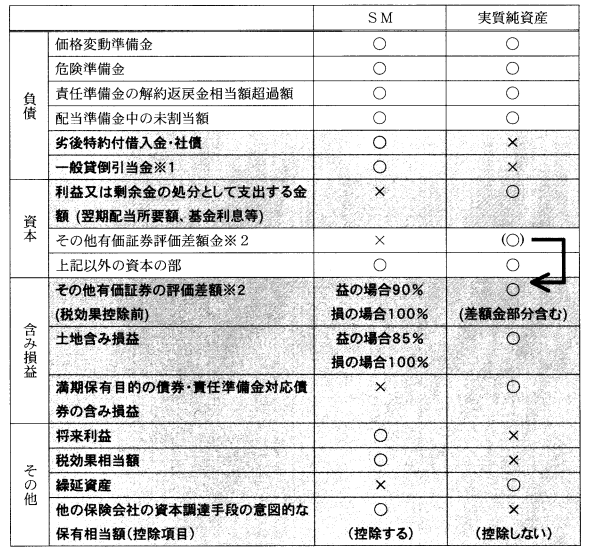
\includegraphics[scale=0.8]{./images/ProbH16-2-3-SMandNetAsset.png}

% \begin{tabularx}{\textwidth}{|c|X|c|c|}
%  \hline
% \multicolumn{2}{c}{} &SM &実質純資産 \\ \hline
% \multirow{6}{*}{負債}&価格変動準備金 &◯& ◯\\ \cline{2-4}
% &危険準備金 &◯& ◯\\ \cline{2-4}
% &責任準備金の解約返戻金相当額超過額 &◯& ◯\\ \cline{2-4}
% &配当準備金中の未割当額 &◯& ◯\\ \cline{2-4}
% &劣後特約付借入金・社債 &◯& ×\\ \cline{2-4}
% &一般貸倒引当金※1 &◯& ×\\ \hline
% \multirow{3}{*}{資本}&利益又は剰余金の処分として支出する金額(翌期配当所要額、基金利息等) &×& ◯\\ \cline{2-4}
% &その他有価証券評価差額金※2 &×& (◯)\\ \cline{2-4}
% &上記以外の資本の部 &◯& ◯\\ \hline
% \multirow{3}{*}{含み損益}&その他有価証券の評価差額※2(税効果控除前) &益の場合90\%損の場合100\%& ◯ (差額金部分含む)\\ \cline{2-4}
% &土地含み損益 &益の場合85\%損の場合100\%& ◯\\ \cline{2-4}
% &満期保有目的の債券・責任準備金対応債券の含み損益 &×& ◯\\ \hline
% \multirow{4}{*}{その他}&将来利益 &◯& ×\\ \cline{2-4}
% & 税効果相当額 &◯& ×\\ \cline{2-4}
% &繰延資産 &×&◯\\ \cline{2-4}
% &他の保険会社の資本調達手段の意図的な保有相当額(控除項目) &◯(控除する)&×(控除しない)\\ \hline
% \end{tabularx}

※1資産の部にマイナス計上される。

※2それぞれ差があるということではなく、合計ではほぼ同じ(違いは益の場合の10%部分のみ)


○上記を踏まえると、当問に対する解答は以下の通りとなる。

○ソルベンシー・マージン総額には含まれるが、実質資産負債差額には含まれない項目

・劣後特約付借入金・社債

・一般貸倒引当金

・将来利益

・税効果相当額

○ソルベンシー・マージン総額には含まれないが、実質資産負債差額には含まれる項目

・資本の部の内、利益または剰余金の処分として支出する金額(翌期配当所要額、基金利息等)

・その他有価証券について含み益がある場合、含み益の90%を超える部分

・土地について含み益がある場合、含み益の85%を超える部分

・満期保有目的の債券・責任準備金対応債券の評価損益

・繰延資産

・他の保険金杜の資本調達手段の意図的な保有相当額

○上記の列挙だけでなく、各項目の簡単な説明や、ソルベンシー・マージンが一般的には事業の
継続的運営を行うためのリスク対応力を表しているのに対し、実質資産負債差額はある時点に
おける清算価値的な純資産の価値を表していること、などを併せて解答することが望ましい。


(2)生命保険会社における早期是正措置制度に関し、以下の事務ガイドラインの導入された目的につ
いて、下線部に注意しながら簡潔に説明せよ。

◯「保険業法第132条第2項に規定する区分等を定める命令」では、実質資産負債差額がマイナス
となった場合には、ソルベンシー・マージン比率がマイナスとなった場合と同様に、早期是正措
置(業務の全部または一部の停止)を内閣総理大臣は命じることができる。これは、ある保険会
社を実質資産負債差額という一つの基準で見て債務超過になっているかどうかを判断し、必要に
応じ措置命令を講じるという趣旨である。

◯しかしながら、実質資産負債差額における資産および負債の評価については、有価証券や土地な
どの資産が時価評価され、負債のほとんどがロック・インされた基礎率に基づく責任準備金であ
る。このため、金利上昇時などには、資産価値が減少する一方、責任準備金の評価額は影響を受
けないため実質資産負債差額がマイナスになる可能性がある。

◯一方で、保険契約は長期にわたる債務であり、ALM管理により資産と負債のバランスが適正に
保たれているのであれば、一時的な金利状況に伴う見かけ上の「債務超過」により保険会社の破綻
を断ずることは不適切であるといえる。

○責任準備金対応債券は、資産・負債のデュレーションマッチングを図り、資産・負債の金利リス
ク変動を適切に管理する際に、保険会社が一定条件を満たした場合、貸借対照表において償却原
価で評価することを認めたものである。今回のガイドラインに規定された満期保有目的の債券と
あわせて、負債の特性に応じて金利変動リスクを軽減するような資産運用を行っている場合につ
いても、日本における責任準備金評価の手法(ロック・イン方式)によって、資産・負債間にお
いて見かけ上ミスマッチが発生し「債務超過」と見えてしまうのは本末転倒である。

○ただし、金利上昇時には、他の金融商品との相対的な比較が行われ、解約が発生することにより
資金流出のおそれもあることから、これに十分対応できる流動性は必須である。

○問題に示されたガイドラインは、上記を踏まえ、

a)実質資産負債差額から、満期保有目的の債券及び責任準備金対応債券の時価評価額と帳簿価
額の差額を除いた額が正の値となり、かつ、

b)流動性資産が確保されている場合

には、実質資産負債差額がマイナスとなっていたとしても、これだけをもって健全性が維持さ
れていないとは判断しないことを明確化したものである。

○当該ガイドラインの効果としては、

・保険会社の資産運用について、負債の特性に応じたものとする際に生じる懸念のあった制約を
排除することが可能となった(当該ガイドラインが明らかにされるまでは、現在のような超低
金利下において、しかも今後金利の先高感がある中で、実質資産負債差額がマイナスにならな
いように資産運用が金利変動を過度に意識した(例えば、あまり長期の債券は購入しない)な
ど、短期的な視点での資産運用とせざるをえないのではないかとの懸念があった。)

・実質資産負債差額の特性について、(マスコミや契約者などの)一般的な理解が進む一つの材料
となったこと

などが挙げられる。

○
なお、解答として求めるものではないが参考として、当該事務ガイドライン改正時の金融庁のプレス発
表資料「事務ガイドライン(「金融監督にあたっての留意事項について(第二分冊:保険会社関係)」)
の一部改正について」(平成15年12月24日)
(http://www.fsa.go.jp/news/newsj/15/hoken/f-20031224-2.html)には以下のとおり記載されている。
「保険会社が債券の長期保有等により適切なALM管理を行っているにも関わらず、金利上昇の結
果、実質資産負債差額が負の値となった場合には、実質資産負債差額から満期保有目的債券及び責
任準備金対応債券の含み損を除いた額が正の値となり、かつ、ALMを維持するに十分な流動性資
産が確保されている場合には、原則として業務停止命令は発出しないこと等を明確化する。」

\problem{H19 生保2問題 1(2)}

実質資産負債差額算出及び 3 号収支分析の「債務超過判定」に関し、以下の空欄を埋めよ。
3 号収支分析の「債務超過判定(事業継続基準の確認)」に係る「資産額」や「負債額」の定義は、
「保険業法第 132 条第 2 項に規定する区分等を定める命令」第 3 条や「平成11年金融監督庁・大蔵
省告示第 2 号」に規定される実質資産負債差額算出における「資産額」や「負債額」の定義とは若干
の相違がある。これを併せて表にまとめると以下のようになる。

\begin{tabularx}{\textwidth}{|X|X|X|}
\hline
 &資産額&負債額\\ \hline
 第132条第2項関係& 「時価評価資産額(満期保有目的債券等も時価評価)」\par 
- 「繰延税金資産(その他有価証券の評価差額が\framebox[3zw]{①}のときの計上金額)」
& 「負債の部計上額」\par - [「\framebox[3zw]{②}」+「危険準備金」\par 
+ 「責任準備金(危険準備金を除く)の解約返戻金相当額[注]超過額」\par 
+ 「配当準備金未割当額」\par  +「繰延税金負債 (その他有価証券の評価差額が\framebox[3zw]{③}のときの計上金額)」]
\\ \hline
3号収支分析 & 「時価評価資産額(満期保有目的債券等も時価評価)」\par 
- 「繰延税金資産(その他有価証券の評価差額が\framebox[3zw]{①}のときの計上金額)」\par 
- 「\framebox[3zw]{④}相当額」
& 「負債の部計上額」\par 
+「解約返戻金相当額[注]」\par 
- [「危険準備金を含んだ責任準備金」\par 
+  「\framebox[3zw]{②}」\par 
+ 「配当準備金未割当額」\par  
+「繰延税金負債 (その他有価証券の評価差額が\framebox[3zw]{③}のときの計上金額)」]
+「\framebox[3zw]{⑤}」
\\ \hline
\end{tabularx}
[注] 全期チルメル式責任準備金と比較しいずれか大きい方の額を計算したもの

\answer{}
① マイナス ② 価格変動準備金 ③ プラス ④ 資産運用リスク ⑤ 劣後特約付債務

\problem{H26 生保2問題 2(2)}
生命保険会社を対象とした早期是正措置制度の概要について、簡潔に説明しなさい。なお、ソルベ
ンシー・マージン比率、実質資産負債差額の計算の詳細については言及する必要はない。

\answer{}
・生命保険会社を対象にした早期是正措置については、生命保険会社の業務の適切な運営を確保し、
契約者保護を図ることを目的として導入された。

・生命保険会社のソルベンシー・マージン比率が200%を下回った場合には、その状況に応じて
監督当局が業務の改善などの命令を発動することで、早期に経営改善への取組みを促していこう
とする制度であり、ソルベンシー・マージン比率の区分に応じて、次のとおり措置内容が定めら
れている。
\begin{tabularx}{\textwidth}{|c|c|X|}
\hline
 区分&ソルベンシー・\par マージン比率&措置の内容\\ \hline
 非対象区分& 200\%以上&なし\\ \hline
 第一区分& 100\%以上\par 200\%未満&経営の健全性を確保するための合理的と認められる改善計画の提出の求め及びその実行の命令\\ \hline
第二区分& 0\%以上\par 100\%未満&次の保険金等の支払能力の充実に資する措置に係る命令
\begin{enumerate}[(1)]
 \item 保険金等の支払能力の充実に係る合理的と認められる計画の提出及びその実行
 \item 配当の禁止又はその額の抑制
 \item 契約者配当又は社員に対する剰余金の分配の禁止又はその額の抑制
 \item 新規に締結しようとする保険契約に係る保険料の計算の方法の変更
 \item 役員賞与の禁止又はその額の抑制その他の事業費の抑制など
\end{enumerate}\\ \hline
第三区分& 0\%未満&期限を付した業務の全部又は一部の停止の命令\\ \hline
\end{tabularx}

・ソルベンシー・マージン比率が0%未満であっても、資産の額から負債を基礎として計算した額
を差し引いた額(=実質資産負債差額)が正の値となる場合には、第二区分の措置が取られるこ
とがある。

・一方、ソルベンシー・マージン比率が0%を上回っていても、実質資産負債差額が負の値となる
場合には、第三区分の措置が取られることがある。

※この場合、実質資産負債差額から、満期保有目的債券および責任準備金対応債券の時価評価額
と帳簿価額の差額を除いた額が正の値となり、かつ、流動性資産が確保されている場合には、
原則としてこの区分の措置はとられないこととなっている。

・生命保険会社が、第二区分または第三区分に該当したことを知った後、速やかに経営改善計画を
自ら策定し、監督当局に提出した場合で、当該経営改善計画が所要の期間で達成できると見込ま
れる場合は、当該経営改善計画達成後に該当する区分(非対象区分は除く)の措置が取られるこ
とがある。

\problem{2019 生保2問題 1(4)}
ある生命保険株式会社のソルベンシー・マージン比率を計算したい。次の情報をもとに、下表の①
~⑥に当てはまる数値を答えなさい。ただし、計算過程においては端数処理を行わず、解答において
は①~⑤は百万円未満を四捨五入して百万円単位、⑥は%未満を四捨五入して%単位とすること。な
お、記載のない項目は考慮する必要はない。
\\[2zh] 
\begin{tabular}{|l|r|}
\multicolumn{2}{r}{ (単位: 百万円, \%)}\\
\hline
ソルベンシー・マージン総額 & 40,020\\ \hline
リスクの合計額 & \framebox[5zw]{  ?}\\ \hline
\ 保険リスク相当額 & \framebox[5zw]{①}\\ \hline
\ 第三分野保険の保険リスク相当額 & \framebox[5zw]{②}\\ \hline
\ 予定利率リスク相当額 & \framebox[5zw]{③}\\ \hline
\ 最低保証リスク相当額 & 1,050\\ \hline
\ 資産運用リスク相当額 & \framebox[5zw]{④}\\ \hline
\ 経営管理リスク相当額 & \framebox[5zw]{⑤}\\ \hline
ソルベンシーマージン比率 & \framebox[5zw]{⑥} \\ \hline
\end{tabular}
\\[2zh] 

\begin{tabularx}{\textwidth}{lrlr}
\multicolumn{2}{l}{(ある生命保険株式会社に関する情報)} & \multicolumn{2}{r}{(単位:百万円)}\\
 普通死亡リスク相当額& 1,824&価格変動等リスク相当額& 6,770\\
 生存保証リスク相当額& 760&責任準備金額(予定利率4\%)& 160,000\\
 災害入院リスク相当額& 1,296& 繰越利益剰余金& 1,000\\
 疾病入院リスク相当額& 1,728&&\\
 再保険リスク相当額& 956&&\\
\end{tabularx}
\\[2zh] 

なお、予定利率リスク相当額の算出にあたって、必要であれば次の表を利用すること。

\begin{tabular}{|c|l|}
 \hline
予定利率の区分& リスク係数\\ \hline
  0.0\%以下の部分& 0.0\\ \hline
  0.0\%を超え 1.5\%以下の部分& 0.01\\ \hline
  1.5\%を超え 2.0\%以下の部分& 0.2\\ \hline
  2.0\%を超え 2.5\%以下の部分& 0.8\\ \hline
  2.5\%を超える部分& 1.0\\ \hline
\end{tabular}

\answer{}
①  保険リスク(相当額,以下省略)は死亡リスクと生存リスクを相関係数を0として合計する\par
$\sqrt{(1824^2+760^2)}=1976$ 百万円 

② 第三分野は災害入院・疾病入院を単純合計する\par
$1296+1728=3024$ 百万円 

③ 予定利率リスクはリスク係数表(0に近い低利率部分は小さく評価する)に従って予定利率を変換し、責任準備金額にかける\par
$1.5\%\times 0.01+(2.0\% -1.5\%)\times 0.2+(2.5\% - 2.0\%)\times 0.8+(4.0\%-2.5\%)\times 1.0 = 0.02015$\par
$160000\times 0.02015=3224$ 百万円 
\\[1zh]
(最低保証リスクは与えられている。保険商品の設計に依存するためか.)

④ 資産運用リスクは、再保険リスクと価格変動等リスクの合計\par
$956+6770=7726$ 百万円 

⑤ 経営管理リスクは、保険リスク + 第三分野保険の保険リスク + 予定利率リスク + 最低保証リスク + 資産運用リスクの合計に 0.02 かける.\par
$(1976+3024+3224+1050+7726)\times 0.02 = 340$ 百万円 

⑥ SM比率は分子はSM総額, 分母は(保険リスク+第三分野リスクの和)と(予定利率リスク+最低保証リスク+資産運用リスク)を相関係数を0として合計したものの1/2と経営管理リスクの単純合計として計算する\par
$$
\frac{40020}{\frac{1}{2}(\sqrt{(1976+3024)^2+(3224+1050+7726)^2}+340)}=600\%
$$

\problem{H24 生保2問題 1(4)}

ある生命保険会社の有価証券の保有目的区分別内訳は表Ⅰのとおりであった。これに基づいて表Ⅱ
のソルベンシー・マージン比率について、以下の①〜⑤の空欄に当てはまる適切な数字を記入しなさ
い。ただし、計算過程および①〜③、⑤の解答においては端数処理を行わず、④の解答においては%
表示で小数点以下第2位を切り捨てて小数点以下第1位まで求めることとする。

\begin{tabular}{|c|r|r|r|}
 \multicolumn{2}{l}{【表Ⅰ保有目的区分内訳】}  & \multicolumn{2}{r}{ (単位: 億円)}\\ \hline
 &帳簿価額&時価&評価差額\\ \hline
満期保有目的の債券& 900 & 1,100& 200\\ \hline
責任準備金対応債券& 30,000 & 32,000& 2,000\\ \hline
その他有価証券& 5,500 & 5,000& -500\\ \hline
合計 & 36,400 & 38,100& 1,700\\ \hline
\end{tabular}

\begin{tabular}{|l|l|l|l|r|}
 \multicolumn{4}{l}{【表Ⅱソルベンシー・マージン比率】}  &  \multicolumn{1}{l}(単位: 億円)\\ \hline
 \multicolumn{4}{|l|}{ソルベンシー・マージン総額} & ***\\ \cline{2-5}
& \multicolumn{3}{|l|}{資本金又は基金等、若しくは供託金等 (外国保険会社等)} & 1,000\\ \cline{2-5}
& \multicolumn{3}{|l|}{価格変動準備金} & 200\\ \cline{2-5}
& \multicolumn{3}{|l|}{危険準備金} & 300\\ \cline{2-5}
& \multicolumn{3}{|l|}{一般貸倒引当金} & 50\\ \cline{2-5}
& \multicolumn{3}{|l|}{その他有価証券評価差額 (税効果控除前) (90\%又は100\%)} &①\\ \cline{2-5}
& \multicolumn{3}{|l|}{土地の含み損益 (85\%又は100\%)} &0\\ \cline{2-5}
& \multicolumn{3}{|l|}{配当準備金未割当部分} & 50\\ \cline{2-5}
& \multicolumn{3}{|l|}{持込資本金等 (外国保険会社等)} & 0\\ \cline{2-5}
& \multicolumn{3}{|l|}{繰延税金資産の不算入額 (-)} & 0\\ \cline{2-5}
& \multicolumn{3}{|l|}{税効果相当額} & 120\\ \cline{2-5}
& \multicolumn{3}{|l|}{負債性資本調達手段等、保険料積立金等余剰部分} & *** \\ \cline{3-5}
&& \multicolumn{2}{l|}{保険料積立金等余剰部分} & 600 \\ \cline{3-5}
&& \multicolumn{2}{l|}{負債性資本調達手段等} & 500 \\ \cline{4-5}
&&& \multicolumn{1}{|l|}{期限付劣後債務} & 500 \\ \cline{4-5}
&&& \multicolumn{1}{|l|}{特定負債性資本調達手段} & 0 \\ \cline{3-5}
&& \multicolumn{2}{l|}{不算入額 (-)} & ② \\ \cline{2-5}
& \multicolumn{3}{|l|}{控除項目 (-)} & 0 \\ \cline{1-5}
 \multicolumn{4}{|l|}{リスクの合計額} & ***\\ \cline{2-5}
& \multicolumn{3}{|l|}{保険リスク相当額} & 350\\ \cline{2-5}
& \multicolumn{3}{|l|}{第三分野保険の保険リスク相当額} & 150\\ \cline{2-5}
& \multicolumn{3}{|l|}{予定利率リスク相当額} & 200\\ \cline{2-5}
& \multicolumn{3}{|l|}{資産運用リスク相当額} & ***\\ \cline{3-5}
&& \multicolumn{2}{l|}{価格変動等リスク相当額} & ③ \\ \cline{3-5}
&& \multicolumn{2}{l|}{信用リスク相当額} & 0 \\ \cline{3-5}
&& \multicolumn{2}{l|}{信用スプレッドリスク相当額} & 0 \\ \cline{3-5}
&& \multicolumn{2}{l|}{子会社等リスク相当額} & 0 \\ \cline{3-5}
&& \multicolumn{2}{l|}{デリバティブ取引リスク相当額} & 0 \\ \cline{3-5}
&& \multicolumn{2}{l|}{再保険リスク相当額} & 0 \\ \cline{3-5}
&& \multicolumn{2}{l|}{再保険回収リスク相当額} & 0 \\ \cline{2-5}
& \multicolumn{3}{|l|}{最低保証リスク相当額} & 0\\ \cline{2-5}
& \multicolumn{3}{|l|}{経営管理リスク相当額} & ***\\ \cline{1-5}
 \multicolumn{4}{|l|}{ソルベンシー・マージン比率 } & ④\\ \cline{1-5}
 \multicolumn{5}{c}{  }\\\cline{1-5}
 \multicolumn{4}{|l|}{中核的支払余力(コア・マージン比率)} & ⑤\\ \cline{1-5}
\end{tabular}

・繰越利益剰余金(相互会社にあっては、当期未処分剰余金)はプラスであったものとする。

・価格変動等リスクの対象となる資産は表Ⅰの有価証券のみであり、すべて邦貨建債券であるものと
する。

・法定実効税率は 30\%とする。

\problem{H14 生保2問題 1(5)}
次の表は、ある生命保険相互会社のある事業年度末における貸借対照表計上額等の諸数値(表中か
ら推計できない項目の金額は 0 とする。)である。この会社の当該事業年度末における「ソルベンシ
ー・マージン比率」(保険金等の支払能力の充実の状況を示す比率)を計算せよ。なお、解答の単位
は%とし、小数点以下第 2 位を四捨五入して小数点以下第 1 位まで求め、その計算過程についても記
載すること。

\begin{tabular}{|l|r|l|r|l|r|}
\multicolumn{4}{l}{   }&\multicolumn{2}{r}{(単位: 百万円)}\\  \hline
項目&金額& 項目&金額& 項目&金額 \\ \hline
 貸倒引当金& 250& 支払備金& 950& その他有価証券評価差額金$^{(*3)}$& 1,200\\ \hline
 \ うち一般貸倒引当金& 100& \ うちIBNR備金& 250&土地含み損益& 200\\ \hline
 繰延税金資産& 1,300&責任準備金 $^{(*2)}$& 97,000& 保険料積立金等余剰部分& 1,500\\ \hline
 純資産の部合計& 3,500& \   うち保険料積立金& 93,500&期限付劣後債務$^{(*4)}$& 300\\ \hline
 \ うち剰余金処分流出額$^{(*1)}$& 650& \ うち未経過保険料& 2,900&税効果相当額& 900\\ \hline
 社員配当平衡積立金& 500& 社員配当準備金& 2,100 &&\\ \hline
 危険準備積立金& 700& \ うち未払・積立配当& 2,000 &&\\ \hline
評価差額金& 800& \ うち未割当額& 100 & 保険リスク相当額$^{(*5)}$ & 700\\ \hline
 当期未処分剰余金& 1,100& 退職給付引当金& 1,200&予定利率リスク相当額& 500\\ \hline
 当期剰余& 750&価格変動準備金& 500&資産運用リスク相当額& 2,000\\ \hline
\end{tabular}

※1:「剰余金処分流出額」中、社員配当準備金(繰入額)は翌期配当所要額と同額である。

※2:「責任準備金」のうち「払戻積立金」は 0 とする。

※3:「その他有価証券評価差額」は税効果控除前の金額である。

※4:契約時における償還期間は5年を超えているものとする。

※5:第三分野保険の保険リスク相当額を含むものとする。

※6:法定実効税率は 30\%とする。

\answer{}

[計算過程]\\
ソルベンシー・マージンの総額\\
= ① (資本の部合計 [3,500] - 剰余金処分流出額 [650] - 評価差額金 [800])\\
+ ②価格変動準備金 [500] + ③危険準備金 [97,000−93,500−2,900]\\
+ ④一般貸倒引当金 [100] + ⑤その他有価証券評価差額 [1,200] × 90%\\
+ ⑥土地含み損益 [200]×85% + ⑦解約返戻金相当額超過部分 [1,500]\\
+ ⑧配当準備金中の未割当額 [100] + ⑨将来利益 [300] + ⑩税効果相当額 [900]\\
= ①2,050 + ②500 + ③600 + ④100 + ⑤1,080 + ⑥170 + ⑦1,500\\
+ ⑧100 + ⑨300 + ⑩900\\
= ⑪\underline{7,300百万円}

 リスクの合計額\\
 =√ \{⑫保険リスク [700] $^2$ + ⑬ (予定利率リスク [500] + 資産運用リスク [2,000])$^2$\}\\
  + ⑭経営管理リスク [ (700 + 500 + 2,000)×2%]\\
 = \{√ (⑫490,000 + ⑬6,250,000) \} + ⑭64\\
 = ⑮ \underline{2,660.151百万円}\\
 したがって、\\
 ソルベンシー・マージン比率 = 100×⑪/ (1/2×⑮) = 548,841…% → \underline{548.8%}


\problem{H19 生保2問題 1(3)}
以下の条件の下で、ソルベンシー・マージン基準におけるリスク相当額を算出せよ。
解答にあたっては計算過程も記載せよ。

\begin{tabular}[b]{|l|l|r|}
 \hline
\multicolumn{2}{|l|}{危険準備金Ⅰ積立限度額}& 700 \\ \cline{2-3}
 &うち普通死亡リスク & 400 \\ \cline{2-3}
 &うち生存保証リスク & 300 \\ \cline{1-3}
\multicolumn{2}{|l|}{危険準備金Ⅱ積立限度額}& 1,250 \\ \cline{2-3}
 &うち予定利率リスク & 250 \\ \cline{2-3}
 &うち責任準備金の3\% & 1,000 \\ \cline{1-3}
\multicolumn{2}{|l|}{資産運用リスク}& 200 \\ \cline{1-3}
\end{tabular}\ \ \ \
\begin{tabular}[b]{|l|l|r|}
\multicolumn{3}{r}{ (単位:百万円)} \\
\hline
\multicolumn{2}{|l|}{最低保証リスク}& 50 \\ \cline{1-3}
\multicolumn{2}{|l|}{危険準備金Ⅳ積立限度額}& 1,600 \\ \cline{2-3}
 &\multirow{2}{*}{うちストレステストの\par  対象とするリスク }& \multirow{2}{*}{1,000} \\ &&\\ \cline{2-3}
 &うち災害死亡リスク & 50 \\ \cline{2-3}
 &うち災害入院リスク & 150 \\ \cline{2-3}
 &うち疾病入院リスク & 400 \\ \cline{1-3}
\end{tabular}

(注)\par
・当該生命保険会社の繰越利益剰余金(相互会社にあっては、当期未処分剰余金)はプラスであ
ったものとする。

・普通死亡リスク、生存保障リスク、災害死亡リスク、災害入院リスク、疾病入院リスク相当額
は、上記の各積立限度額と一致するものとする。

\answer{}

保険リスク $R_1=\sqrt{400^2+300^2}=500$\\
保険リスクは, 死亡と生存を相関係数0で合算する

第三分野の保険リスク $R_8=1000/10+50+150+400=700$\\
第三分野は, ストレステストの対象は/10し、それ以外はそのまま単純合計する

経営管理リスク $R_4=(500+250+200+50+700)\times 0.02=34$\\
経営管理リスクは、保険 (上で求めた), 予定利率, 資産運用, 最低保証, 第三分野の単純合計の2\% 

リスク量 = $\sqrt{(500+700)^2+(250+200+50)^2}+34=1334$\\
リスク量は, (保険+第三分野)と(予定利率+資産運用+最低保証)を相関係数0で合算したものと経営管理の単純合計

\problem{H12 生保2問題 1(2)(3)}
我が国のソルベンシー・マージン基準に関し、次の①~⑤を適当な語句または数値で埋めよ。また、
ソルベンシー・マージン基準における保険リスク相当額を計算しなさい。

\begin{tabular}{|l|l|r|r|}
 \hline
リスクの種類&リスク対象金額&左記実額&リスク係数\\  \hline
&&百万円&\\
 普通死亡リスク& \framebox[2zw]{①}& 10,500,000 & \framebox[2zw]{④}\\ \hline
 災害死亡リスク&災害死亡保険金額& 1,200,000 & 0.06/1,000\\ \hline
 生存保障リスク&個人年金保険\framebox[2zw]{②}& 150,000 & 10/1,000\\ \hline
 災害入院リスク&災害入院日額総額×予定平均給付日数& 3,000 & 3/1,000\\ \hline
 疾病入院リスク&疾病入院日額総額×予定平均給付日数& 4,000 & 7.5/1,000\\ \hline
 その他のリスク& \framebox[2zw]{③} &3,000& \framebox[2zw]{⑤}\\ \hline
\end{tabular}

\answer{}
①危険保険金額②期末責任準備金額
③危険準備金積立限度額
④0.6/1,000⑤1

G.9,585百万円

\answer{H25 生保2問題 1(5)}

次の表1および表2をもとに、実質資産負債差額を算出したい。
表3の空欄 a,b および c の金額を算出しなさい。なお、表 1 および表 2 に記載のない項目は考慮する必要はない。\\

【表1】\\
\begin{tabular}{|l|r|}
\hline 項目&金額\\ \hline \hline
貸借対照表の資産の部合計&49,800\\ \hline
貸借対照表の負債の部合計&47,700\\ \hline
価格変動準備金&400\\ \hline
危険準備金&600\\ \hline
配当準備金中の未割当額&100\\ \hline
解約返戻金相当額※超過部分&1,200\\ \hline
基金&1,000\\ \hline
負債性資本調達手段&600\\ \hline
特定負債性資本調達手段&400\\ \hline
その他&200\\ \hline
一般貸倒引当金&100\\ \hline
その他有価証券に係る繰延税金負債&200\\ \hline
\end{tabular}\\

【表2】\\
\begin{tabular}{|l|r|}
\hline
 項目&金額\\\hline\hline
その他有価証券含み損益&600\\ \hline
満期保有目的債券含み損益&1,000\\ \hline
責任準備金対応債券含み損益&800\\ \hline
土地の含み損益&-100\\ \hline
\end{tabular}\\ 

【表3】\\
\begin{tabular}{|l|r|}
\hline
 (1) 資産の部に計上されるべき金額の合計& a\\ \hline
 (2) 負債の部に計上されるべき金額の合計& b\\\hline
 実質資産負債差額 (1)-(2) & c\\\hline
\end{tabular}

\answer{}

a 51,500
b45,200
c 6,300\\
\begin{tabular}{|l|l|l|r|l}
\cline{1-4}
\multicolumn{3}{|l|}{
(1)資産の部に計上されるべき金額の合計額(=①+②+③+④-⑤)} & 51,500 & a\\ \cline{2-4}
& \multicolumn{2}{l|}{①貸借対照表の資産の部合計} & 49,800 &\\ \cline{2-4}
& \multicolumn{2}{l|}{②有価証券の時価と貸借対照表計上額との差額} & 1,800 &\\ \cline{2-4}
& \multicolumn{2}{l|}{③有形固定資産含み損益} & -100 &\\ \cline{2-4}
& \multicolumn{2}{l|}{④上記以外の資産の含み損益} & &\\ \cline{2-4}
& \multicolumn{2}{l|}{⑤その他有価証券に係る繰延税金資産} & &\\ \cline{1-4}
\multicolumn{3}{|l|}{(2)負債の部に計上されるべき金額の合計額を基礎として計算した金額\par 
(=①-②-③-④-⑤)} & 45,200& b\\ \cline{2-4}
& \multicolumn{2}{l|}{①貸借対照表の負債の部合計} & 47,700 &\\ \cline{2-4}
& \multicolumn{2}{l|}{②価格変動準備金} & 400 &\\ \cline{2-4}
& \multicolumn{2}{l|}{③危険準備金} & 600 &\\ \cline{2-4}
& \multicolumn{2}{l|}{④将来の保険金等の支払に備えて積み立てている準備金の一部} & 1,300 &\\ \cline{3-4}
&& 解約返戻金相当額超過部分(④(a))& 1,200 &\\ \cline{3-4}
&& 配当準備金中の未割当額(④(b))& 100 &\\ \cline{2-4}
& \multicolumn{2}{l|}{⑤その他有価証券に係る繰延税金負債} & 200 &\\ \cline{1-4}
\multicolumn{3}{|l|}{実質資産負債差額 (1)-(2)} & 6,300 & c\\ \cline{1-4}
\end{tabular}\\ \\ \\

参考:実質資産負債差額内訳\\
\begin{tabular}{|l|lc|r|c}
 \cline{1-4}
\multicolumn{2}{|l}{実質資産負債差額の内訳} & & 6,300&c\\ \cline{2-4}
&純資産の部& + & 2,100&\\ \cline{2-4}
&その他有価証券に係る繰延税金資産&-&&\\ \cline{2-4}
&含み損益(満期保有目的債券)&+&1,000&\\ \cline{2-4}
&含み損益(責準対応債券)&+&800&\\ \cline{2-4}
&含み損益(土地)&+&-100&\\ \cline{2-4}
&含み損益(その他)&+&&\\ \cline{2-4}
&その他有価証券に係る繰延税金負債&+&200&\\ \cline{2-4}
&価格変動準備金&+&400&\\ \cline{2-4}
&危険準備金&+&600&\\ \cline{2-4}
&配当準備金中の未割当額&+&100&\\ \cline{2-4}
&解約返戻金相当額超過部分&+&1,200&\\ \cline{1-4}
\end{tabular}

\problem{H25 生保2問題 1(5)}

次の表1および表2をもとに、実質資産負債差額を算出したい。
表3の空欄 a,b および c の金額を算出しなさい。なお、表 1 および表 2 に記載のない項目は考慮する必要はない。

【表1】\\
\begin{tabular}{|l|l|r|}
 \hline
 \multicolumn{2}{|l|}{項目}&金額 \\ \hline
 \hline
 \multicolumn{2}{|l|}{貸借対照表の資産の部合計}&49,800 \\ \hline
 \multicolumn{2}{|l|}{貸借対照表の負債の部合計}&47,700 \\ \hline
 \multicolumn{2}{|l|}{価格変動準備金}&400 \\ \hline
 \multicolumn{2}{|l|}{危険準備金}&600 \\ \hline
 \multicolumn{2}{|l|}{配当準備金中の未割当額}&100 \\ \hline
 \multicolumn{2}{|l|}{解約返戻金相当額※超過部分}&1,200 \\ \hline
 \multicolumn{2}{|l|}{基金}&1,000 \\ \hline
 &負債性資本調達手段& 600\\ \hline
 &特定負債性資本調達手段& 400\\ \hline
 \multicolumn{2}{|l|}{その他}&200 \\ \hline
 \multicolumn{2}{|l|}{一般貸倒引当金}&100 \\ \hline
 \multicolumn{2}{|l|}{その他有価証券に係る繰延税金負債}&200 \\ \hline
\end{tabular}\\

【表2】\\
\begin{tabular}{|l|l|r|}
 \hline
 \multicolumn{2}{|l|}{項目}&金額 \\ \hline
 \hline
 \multicolumn{2}{|l|}{その他有価証券含み損益}&600 \\ \hline
 \multicolumn{2}{|l|}{満期保有目的債券含み損益}&1,000 \\ \hline
 \multicolumn{2}{|l|}{責任準備金対応債券含み損益}&800 \\ \hline
 \multicolumn{2}{|l|}{土地の含み損益}&-100 \\ \hline
 \end{tabular}\\

【表3】\\
\begin{tabular}{|l|c|}
\hline
 (1)資産の部に計上されるべき金額の合計額& a\\ \hline
(2)負債の部に計上されるべき金額の合計額を基礎として計算した金額 & b\\ \hline
 実質資産負債差額 (1)-(2)& c\\ \hline
\end{tabular}

\answer{}

\begin{tabular}{|l|l|l|r|l}
\cline{1-4}
\multicolumn{3}{|l|}{
 (1)資産の部に計上されるべき金額の合計額(=①+②+③+④-⑤)} & 51,500 & a\\ \cline{2-4}
 & \multicolumn{2}{|l|}{①貸借対照表の資産の部合計} & 49,800 &\\ \cline{1-4}
 & \multicolumn{2}{|l|}{②有価証券の時価と貸借対照表計上額との差額} & 1,800 &\\ \cline{2-4}
 & \multicolumn{2}{|l|}{③有形固定資産含み損益} & -100 &\\ \cline{2-4}
 & \multicolumn{2}{|l|}{④上記以外の資産の含み損益} & &\\ \cline{2-4}
 & \multicolumn{2}{|l|}{⑤その他有価証券に係る繰延税金資産} & &\\ \cline{1-4}
\multicolumn{3}{|l|}{
(2)負債の部に計上されるべき金額の合計額を基礎として計算した金額\par 
(=①-②-③-④-⑤)}  & 45,200 & b \\ \cline{2-4}
 & \multicolumn{2}{|l|}{①貸借対照表の負債の部合計} & 47,700 &\\ \cline{2-4}
 & \multicolumn{2}{|l|}{②価格変動準備金} & 400 &\\ \cline{2-4}
 & \multicolumn{2}{|l|}{③危険準備金} & 600 &\\ \cline{2-4}
 & \multicolumn{2}{|l|}{④将来の保険金等の支払に備えて積み立てている準備金の一部} & 1,300 &\\ \cline{3-4}
 & & 解約返戻金相当額超過部分(④(a))& 1,200 &\\ \cline{3-4}
 & & 配当準備金中の未割当額(④(b))& 100 &\\ \cline{2-4}
 & \multicolumn{2}{|l|}{⑤その他有価証券に係る繰延税金負債} & 200 &\\ \cline{1-4}
 \multicolumn{3}{|l|}{実質資産負債差額 (1)-(2)} & 6,300 &c\\ \cline{1-4}
\end{tabular}

参考:実質資産負債差額内訳

\begin{tabular}{|l|lc|r|l}
\cline{1-4}
 \multicolumn{3}{|l|}{実質資産負債差額の内訳}& 6,300&c \\ \cline{2-4}
& 純資産の部 &+ & 2,100&\\ \cline{2-4}
& その他有価証券に係る繰延税金資産 &- & &\\ \cline{2-4}
&  含み損益(満期保有目的債券)&+ & 1,000&\\ \cline{2-4}
&  含み損益(責準対応債券)&+ & 800&\\ \cline{2-4}
&  含み損益(土地)&+ & -100&\\ \cline{2-4}
&  含み損益(その他)&+ & &\\ \cline{2-4}
& その他有価証券に係る繰延税金負債 &+ &200 &\\ \cline{2-4}
&価格変動準備金 &+ &400 &\\ \cline{2-4}
& 危険準備金 &+ &600 &\\ \cline{2-4}
& 配当準備金中の未割当額 &+ &100 &\\ \cline{2-4}
&解約返戻金相当額超過部分 &+ &1,200 &\\ \cline{2-4}
\end{tabular}

\problem{H21 生保2問題 1(3)}
ある決算期において、「その他有価証券」の時価が前期よりも下落した。この場合の影響について、以下の①~⑤の空欄に当てはまる最も適切な語句(例:○○百万円増加/○○百万円減少/増減なし)を記入しなさい。

《前提》\\
その他有価証券の帳簿価額:100 百万円(前期末、当期末とも)\\
その他有価証券の前期末時価:130 百万円\\
その他有価証券の当期末時価:80 百万円\\
その他有価証券は全て邦貨建債券であり、全部純資産直入法で評価。\\
当期の有価証券の売買はなく、また過年度・当期とも減損処理は行っていない。\\
その他有価証券の時価の下落以外の要因による損益・資産・負債の状況は、全て前期(末)と同一。\\
実効税率:40%\\
繰延税金資産は回収可能であり、繰延税金資産を認識する。\\

ア.損益計算書への影響\\
経常利益は、前期と比べ、①。\\
イ.貸借対照表への影響\\
純資産の部におけるその他有価証券評価差額金は、前期末と比べ、②。
ウ.健全性指標への影響\\
実質資産負債差額は、前期末と比べ、③。\\
ソルベンシー・マージン総額は、前期末と比べ、④。\\
エ.剰余金分配等の限度となる額への影響\\
保険業法第 55 条第 2 項に定める剰余金分配の限度となる償却等限度額(相互会社)あるいは会社法第 461 条第 2 項に定める株主配当の分配可能額(株式会社)は、前期末と比べ、⑤。

ただし、損失てん補準備金(相互会社)あるいは利益準備金(株式会社)の当期繰入負担に係る増
減は無視してよい。また、前期末の剰余金分配の限度となる償却等限度額あるいは株主配当の分配可
能額は潤沢にあるものとする。
\answer{}
①増減なし②30百万円減少
③50百万円減少
④47百万円減少
⑤12百万円減少

<解説>
その他有価証券の含み損益部分を抜き出した前期末B/Sおよび当期末B/Sは下記のとおり。

前期末B/S
\begin{tabular}{lrlr}
その他有価証券 & 30 & その他有価証券評価差額金&18\\
 & &繰延税金負債&12 \\
\end{tabular}

当期末B/S
\begin{tabular}{lrlr}
その他有価証券&▲20&その他有価証券評価差額金&▲12\\
繰延税金資産&8\\
\end{tabular}

①全部純資産直入法なので、当期損益計算書への影響はなし。\\
②その他有価証券評価差額金の増減額 = -12 -18 = -30\\
③実質純資産負債差額の増減額\\
=  純資産の部の増減額+繰延税金負債・資産の増減額\\
= その他有価証券評価差額金の増減額+繰延税金負債・資産の増減額\\
=(-12-18)+(-8-12)=-50\\
④ソルベンシー・マージン総額の増減\\
=その他有価証券の評価差額の一定率(税引前)の増減額\\
=-20×100%-30×90%=47 [一定率は、評価差額が正の場合90%、それ以外の場合100%]\\
⑤剰余金分配等の限度となる金額の増減\\
=-12−0[正の評価差額は不算入]

\section{6.3 動的なソルベンシーの検証}
\problem{H30 生保2問題 3(2)①、H24 生保2問題 1(3)}
日本の生命保険会社のソルベンシーについて、静的なソルベンシーの検証・動的なソルベンシーの検証について説明せよ。その他については略(生命保険会社の保険計理人の職務参照)

\answer{}
①
静的なソルベンシーの検証

フォーミュラ方式によるソルベンシー・チェックであり、日本ではソルベンシー・マージン比
率や実質資産負債差額による検証が行なわれている。

保険契約上の債務の履行を確実に行うため、責任準備金だけでなく、責任準備金を超えて保有
する「広義の自己資本(ソルベンシー・マージン)」を用いて評価する。

また、保険会社を取り巻くリスク、もしくは「(広義の)自己資本」で対応するべきリスクを
定量化し、それをもとに、「(広義の)自己資本」の保有基準が定められ、実際の保有度合いの
適正性を測ることが可能。

フォーミュラ方式による検証は、実行可能性や検証可能性に優れており、全ての保険会社を統
一的に取り扱うことが可能なことから、客観的な指標として監督行政に活用されている。

一方、各保険会社固有のリスクが必ずしも反映されないことや、あくまで一時点の検証に過ぎ
ない、といったデメリットがあるため、戦略決定等のための経営管理上の要請には完全には対
応できない。動的なソルベンシーの検証と併せた検証が必要である。

動的なソルベンシーの検証

将来のキャッシュ・フロー分析によるシミュレーションによるソルベンシー検証の方法であり、
静的なソルベンシー検証を補完する位置付けとしての活用が可能である。

日本では保険計理人の実務基準に基づく将来収支分析が規定されているほか、監督指針におい
てストレステストの自主的な実施が求められている。

会社の業務政策、投資戦略、ALM、市場戦略、契約者配当、株主配当等を反映させることに
より、会社固有のリスクに対するソルベンシー確保の検証を行うことができる。

一方、計算実務が繁雑であること、計算結果の説明が必ずしも容易でないこと、モデル・シナ
リオ等の設定における恣意性の排除が難しい側面があること等のデメリットがある。

今後、新しいリスクの出現、新しいアクチュアリアルな技術の開発等の環境や状況の変化に応
じて、継続的にその内容を見直していくことが必要となる。

\section{6.4 支払保証制度}
\problem{2021生保2問題 1(5), H24 生保2問題 1(3)}
支払保証制度(保険会社が経営破綻に陥った場合に、破綻保険会社に代わって保険契約者等に対する債務を履行する機能を有することで、保険契約者等の保護を図る制度)の必要性に関し、監督当局・保険会社・保険契約者等の関係者にとっての、保険契約者の保護を図ること以外のメリットを2つ、および同関係者にとってのデメリットを3つ挙げなさい。
\answer{}

メリット

保険業界自体の信頼性が確保される。

保険会社を絶対に破たんさせない、という監督行政方針が敷かれている場合に比べ、保険会社の自由な競争が促進される。

デメリット

過度な契約者の保護が行われることで、保険会社、保険契約者そして監督当局のモラル・ハザー
ドが誘発されやすくなる。

健全な会社も拠出金を求められることで健全性を損なってしまう危険がある。

規制緩和の流れに逆行し、グローバル・マーケットでの競争条件の不均衡を招く。


\section{6.5 契約条件の変更(試験範囲外)}
(空欄)
\end{document}

